\documentclass{article}
\usepackage{float,amsmath}
\usepackage{graphicx}
\usepackage{color}
\usepackage[letterpaper,margin=1in]{geometry}
\usepackage{hyperref}

%\setlength{\textwidth}{6.5in}

\begin{document}

\author{HERA}
\title{Roadmap for HERA Network Configuration and Bandwidth}
\maketitle

\section{Introduction}
HERA is an international experiment to detect and characterize the Epoch of
Reionization (EOR).  The telescope is located at the South African SKA site in
the Karoo Astronomy Reserve.  This brief summarizes the overall network
configuration and bandwidth for HERA as relevant to the interfaces with SKA-SA
infrastructure.  HERA construction and observing are proceeding in parallel.

The HERA correlator is currently located next to the telescope array. In late 2017 or early 2018, the correlator will be moved to the KAPB. At that time the correlator will ingest raw voltage streams at terabit rates. These will be fed over a bundle of 96 fibers from the array to the KAPB.

\section{Current setup and KAPB move}
Figure~\ref{fig:hi_level} shows the very high-level network configuration for
2017 and 2018.  The correlator currently lives in the `HERA container' in the
middle of the HERA telescope array.  The correlator data files are transferred for processing and storage in the CMC container using a dedicated fiber.  The processed files are then transferred off-continent to the USA, currently to a cluster at the University of Pennsylvania in Philadelphia, PA.  Over the next month or two, the CMC-based equipment will be moved to the KAPB and the USA node will be moved to the National Radio Astronomy Observatory (NRAO) site in Socorro, NM.  The single pair of 1Ge fiber between the HERA container and the processing cluster is adequate for operations through fall of 2017.

\begin{figure}[H]
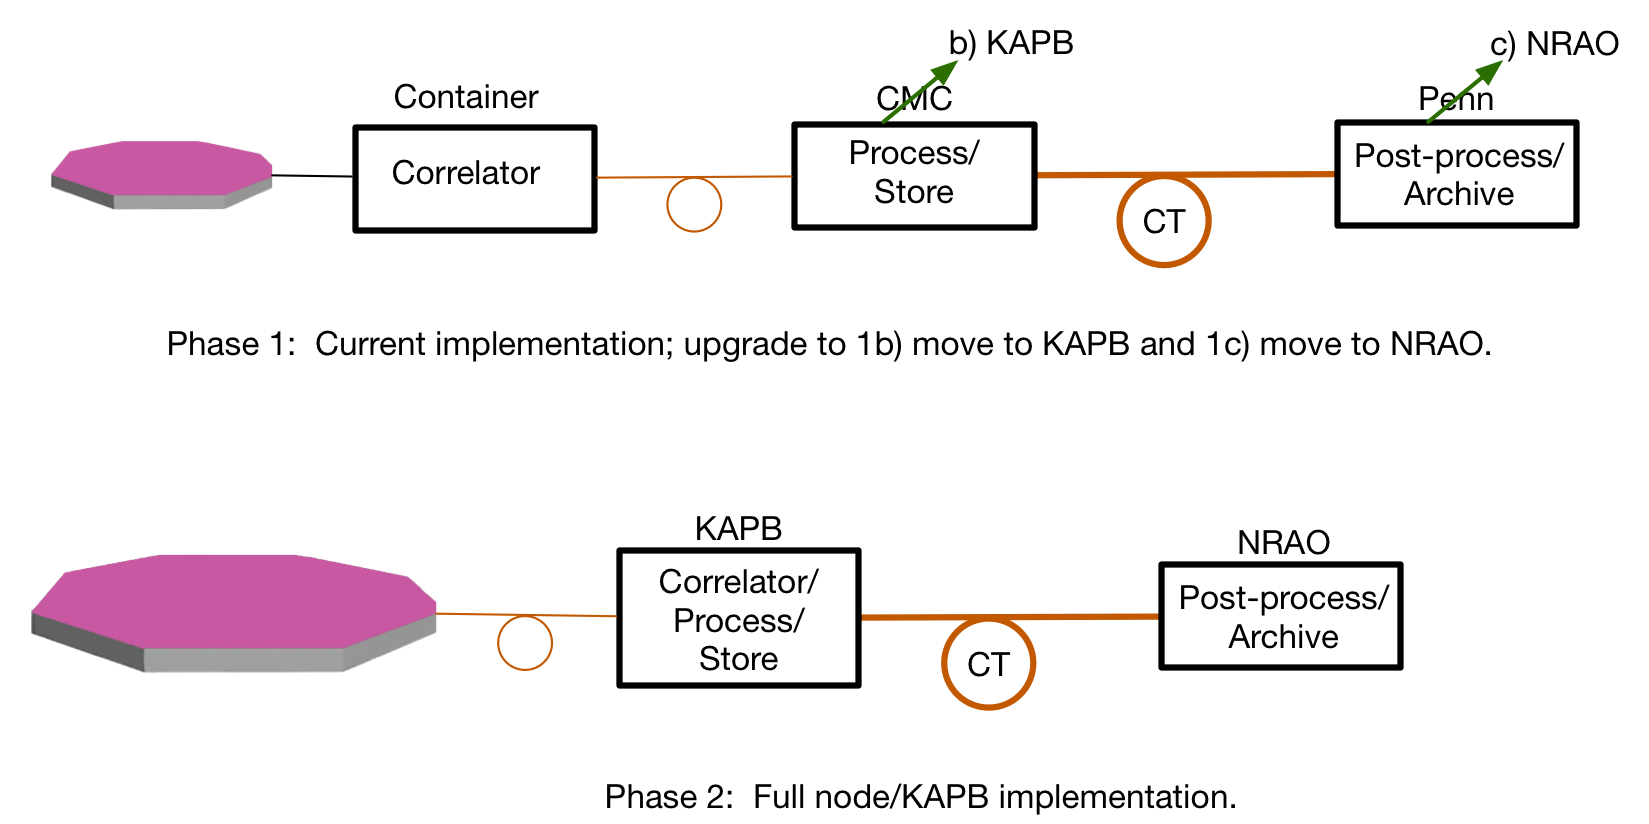
\includegraphics[width=0.8\textwidth]{network.png}
\centering
\caption{High-level organization of network.  See text for explanation.}
\label{fig:hi_level}
\end{figure}

Prior to the move of the equipment from the CMC to the KAPB, there is a desire
to update the network configuration to accommodate the evolving needs of the
KAT/SKA network and HERA.  There is no strict requirement that this must
happen before the physical move, but doing so allows the network change to be
deployed separately from the major hardware relocation.  When the equipment is relocated to the KAPB additional storage will be added to the system and the switches will be upgraded.

Figure~\ref{fig:net_org} shows a schematic of the proposed network arrangement. In order to ensure smooth HERA operations through mid-2018, \textbf{the following requirements must be satisfied:}
\begin{enumerate}
\item There must be a login portal allowing secure access to HERA nodes from the Internet.
\item There must be 32 IP addresses reserved for HERA nodes on the SKA/KAT network so that they may be accessed directly from our login portal.
\item Some HERA nodes must be able to access to the SKA/KAT network for integration with CAM (as both data sinks and data sources).
\item There must be a dedicated fiber pair between the HERA container and the HERA processing cluster (currently located in the CMC; soon KAPB).
\item The network must support a data rate to the US of 200~Mbps by mid-2017, growing to 400~Mbps by mid-2018.
\end{enumerate}

\begin{figure}[H]
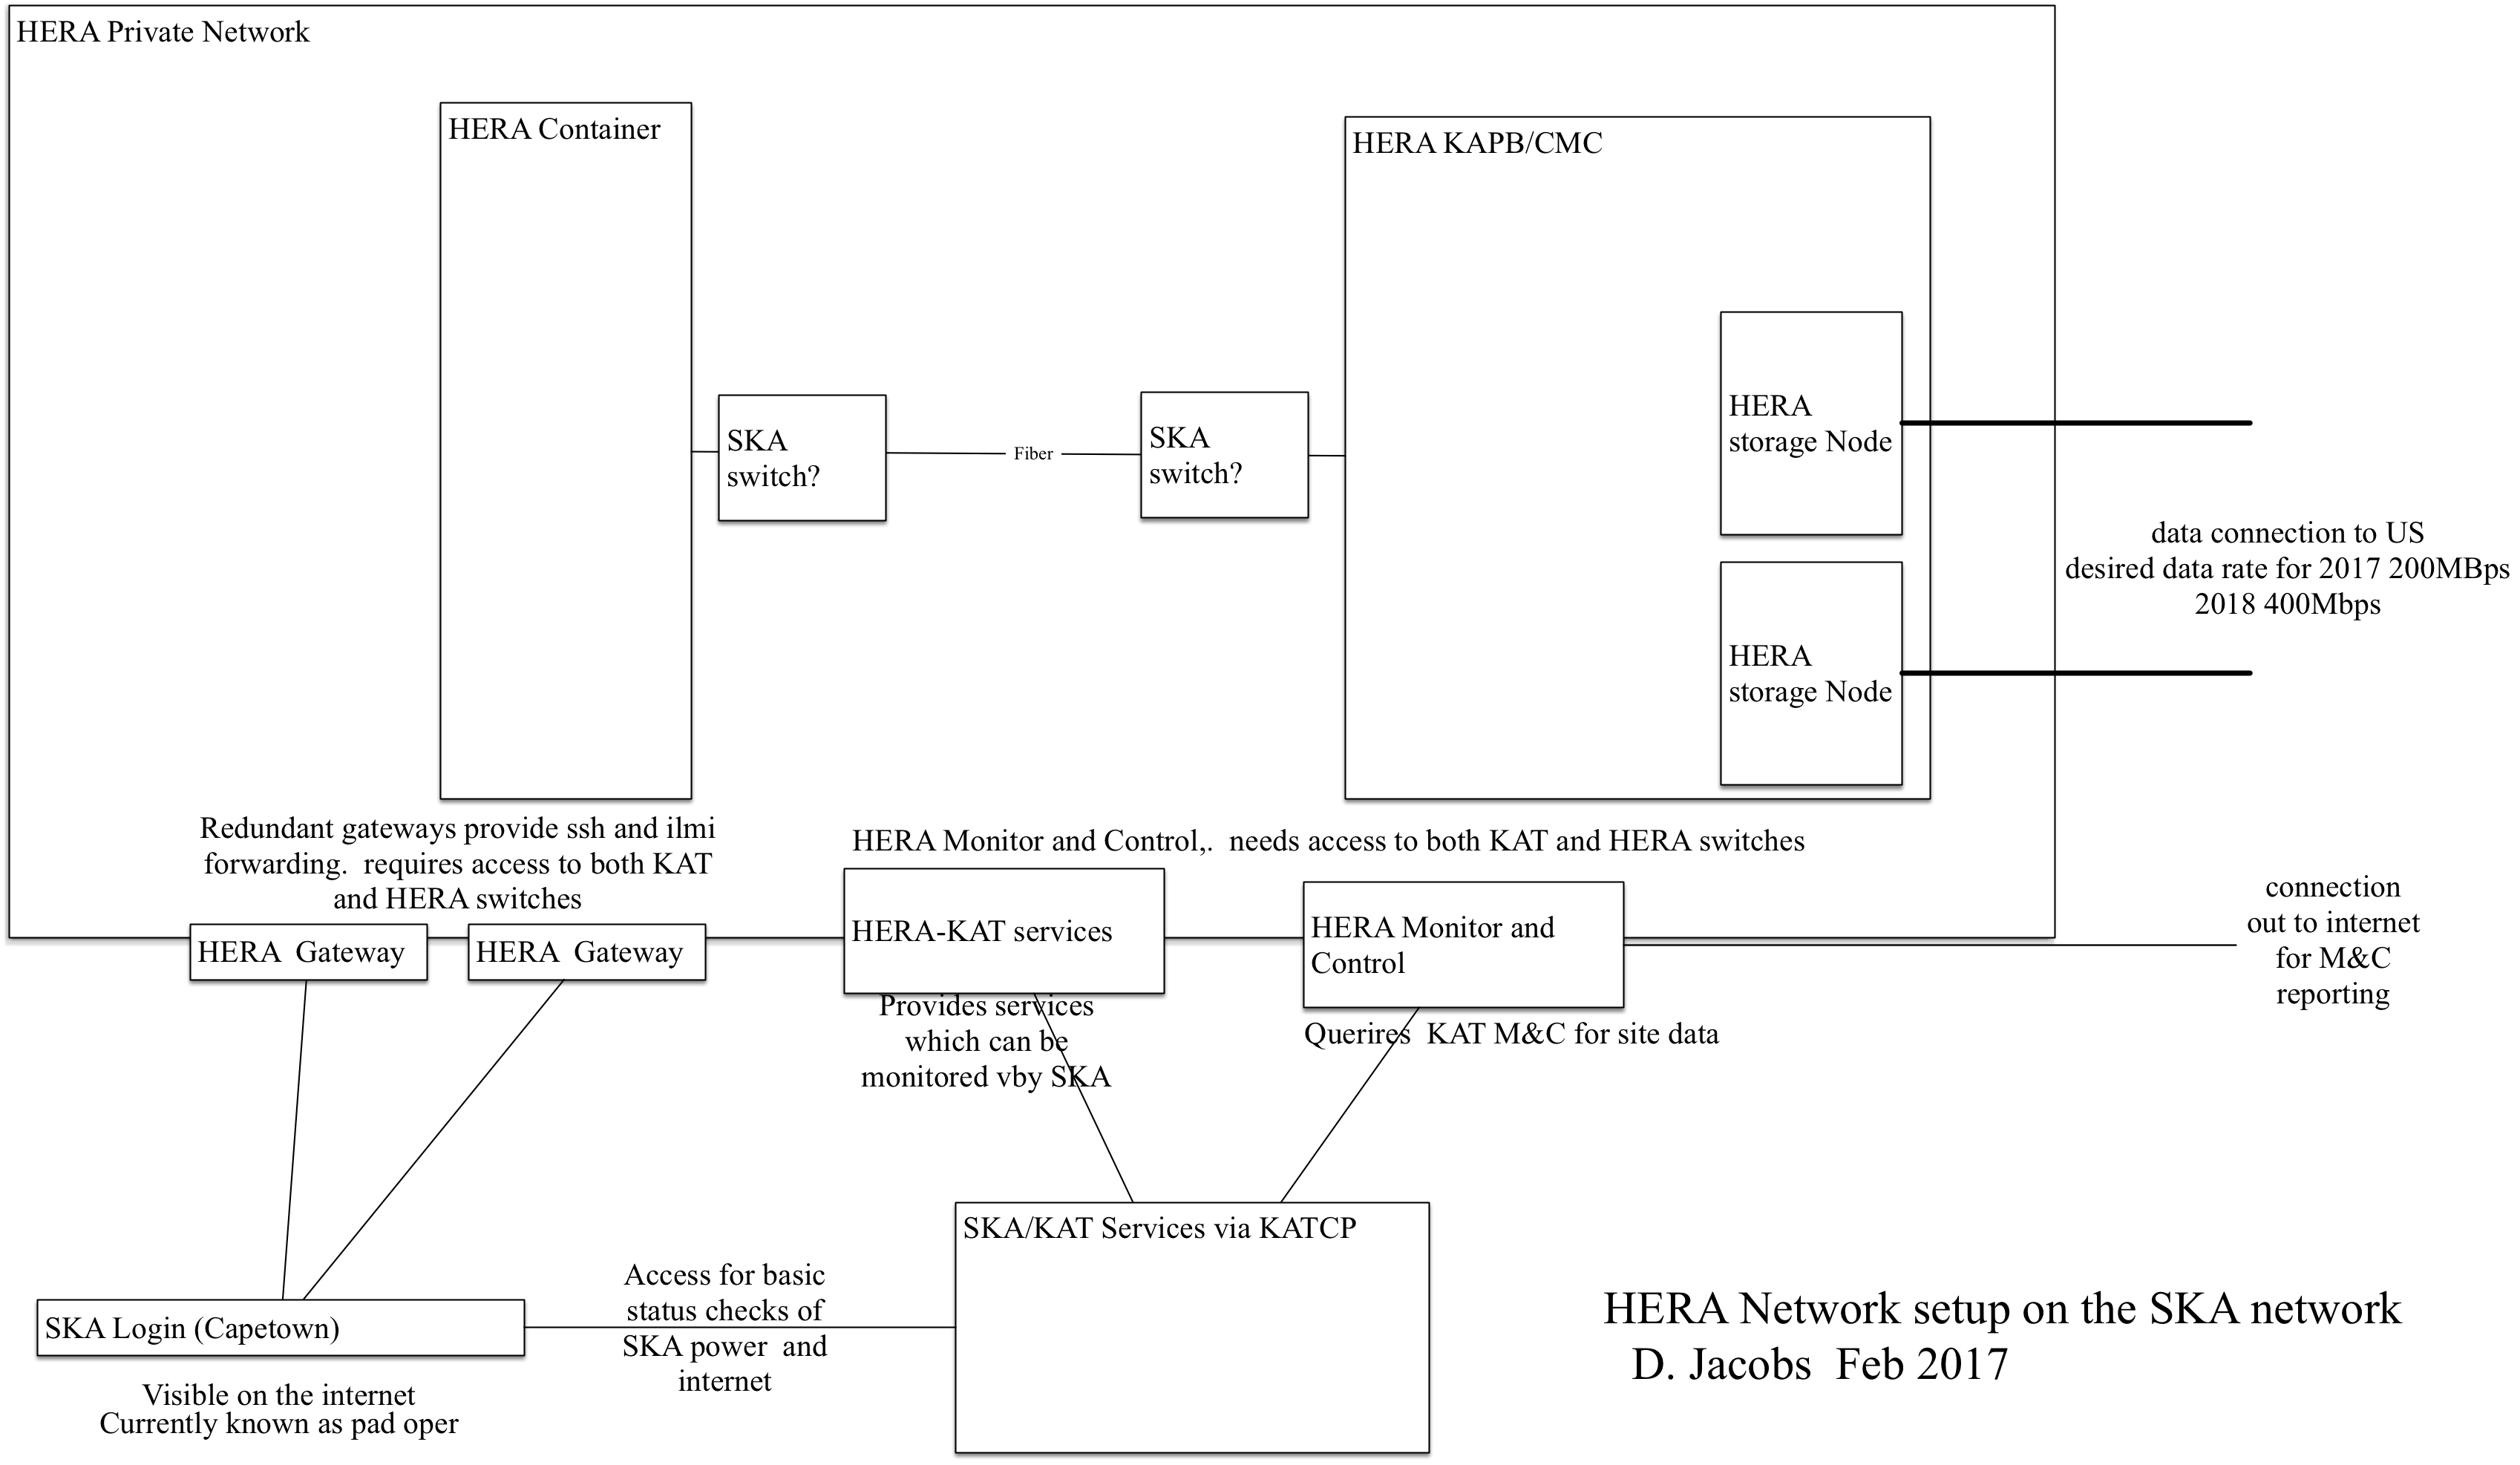
\includegraphics[width=\textwidth]{HERA_2017_network_organization.png}
\centering
\caption{Schematic of proposed network arrangement.}
\label{fig:net_org}
\end{figure}

\section{Data Rate}
HERA currently records at a data rate of 200~Mbps. In 2018 this will increase to 1.5~Gbps. Currently the average bandwidth to the US is 60~Mbps, so we can only transfer a small fraction of our data. This limits analysis capabilities and means that mission-critical data are not replicated off-site. Moving data at the currently-attainable rate of 60~Mbps causes conflict with SKA~SA staff Internet use, so copies to the US are limited to night-time hours, further reducing the effective bandwidth available to the project.

The desired data rate to support current operations is 200~Mbps. The target for mid-2018 is 400~Mbps.

\end{document}
